\section{Introduction}
Once the first version of the automated pipeline was built, we started using it to reduce the ULTRACAM archive. We evaluated some key aspects of the automated pipeline. Whether the photometry it produces is of sufficient quality to allow researchers to view light-curves that clearly demonstrate the astronomical events occuring in the data. We also wanted to see whether the ease of access to the data allowed us to discover new variable objects. Finally, we tried to use the pipeline to process the entire ULTRACAM archive to test if it was robust enough to reduce the data despite the diversity of the inputs. 

\section{Quality of the photometry}
The main purpose of this MSc project was to establish a process for automatically reducing the light-curves for all objects in the data archive rather than trying to produce accurate and well-calibrated measurements. The diverse nature of the dataset means that it is not trivial to write an automated algorithm that can perform fully calibrated measurements. The automated pipeline lacks the ability to correctly identify the appropriate bias readings, flat-fields and standard stars that should be used for photometric calibration. Therefore, this step is skipped altogether. The magnitudes and flux counts produced by the automated pipeline are not calibrated and will differ from their true values by a certain offset. 

\begin{figure}
\centering
\includegraphics[width=120mm]{images/2013-07-13-run111-r-withlabels.png}
\caption{Snapshot taken from the automated pipeline browser for 2013-07-13/run111. The target, {NN Ser} is labeled object `7' and the object we have used as the comparison is labeled '0' in the image. This is a stacked image from the 'red' CCD with the Sloan 'i' filter. }
\label{fig:nnserfield}
\end{figure}

Since the ULTRACAM already has a well-established data reduction pipeline, it is useful to compare the results of this pipeline with the new, automated one built in this project. As mentioned above, the automated pipeline does not perform calibrated photometry, but we can still compare the non-calibrated photometry to get an estimate of how well our new pipeline performs.

In order to do this, we chose a run of a target object that has often been observed with the ULTRACAM. The object is NN Ser, a white-dwarf, M-dwarf eclipsing binary. The specific run in question is \emph{2013-07-13/run111}. Producing the photometry using the automated pipeline on this run is achieved by simply typing: \texttt{runbuilder.py 2013-07-13/run111} on the command line. Please refer to the user manual in appendix \ref{chap:usermanual} for instructions on how to install and run the pipeline.  The reduction takes about 5 minutes to process when running on a standard desktop machine in the University of Warwick Astronomy department. The output of this reduction can be seen at \url{http://deneb.astro.warwick.ac.uk/phrnaw/sitedev/2013-07-13/run111.html}. We also reduced the same run with the traditional pipeline. In both cases we produced light-curves by plotting the relative flux of the target relative to the comparison. In figures \ref{fig:comparepipelines_r} to \ref{fig:comparepipelines_zoom_b} we have plotted the results of the automated pipeline together with the traditional pipeline (with a small offset applied to separate the data points). Inspections of these plots shows that the pipelines produce consistant results. The pipelines seem to have similar RMS scatter and show the same trends. Closer inspection reveals that outlying data points usually occur concurrently demonstrating that the systematic differences between the two approaches are smaller than the intrinsic errors in the measurements. 

\begin{figure}
\centering
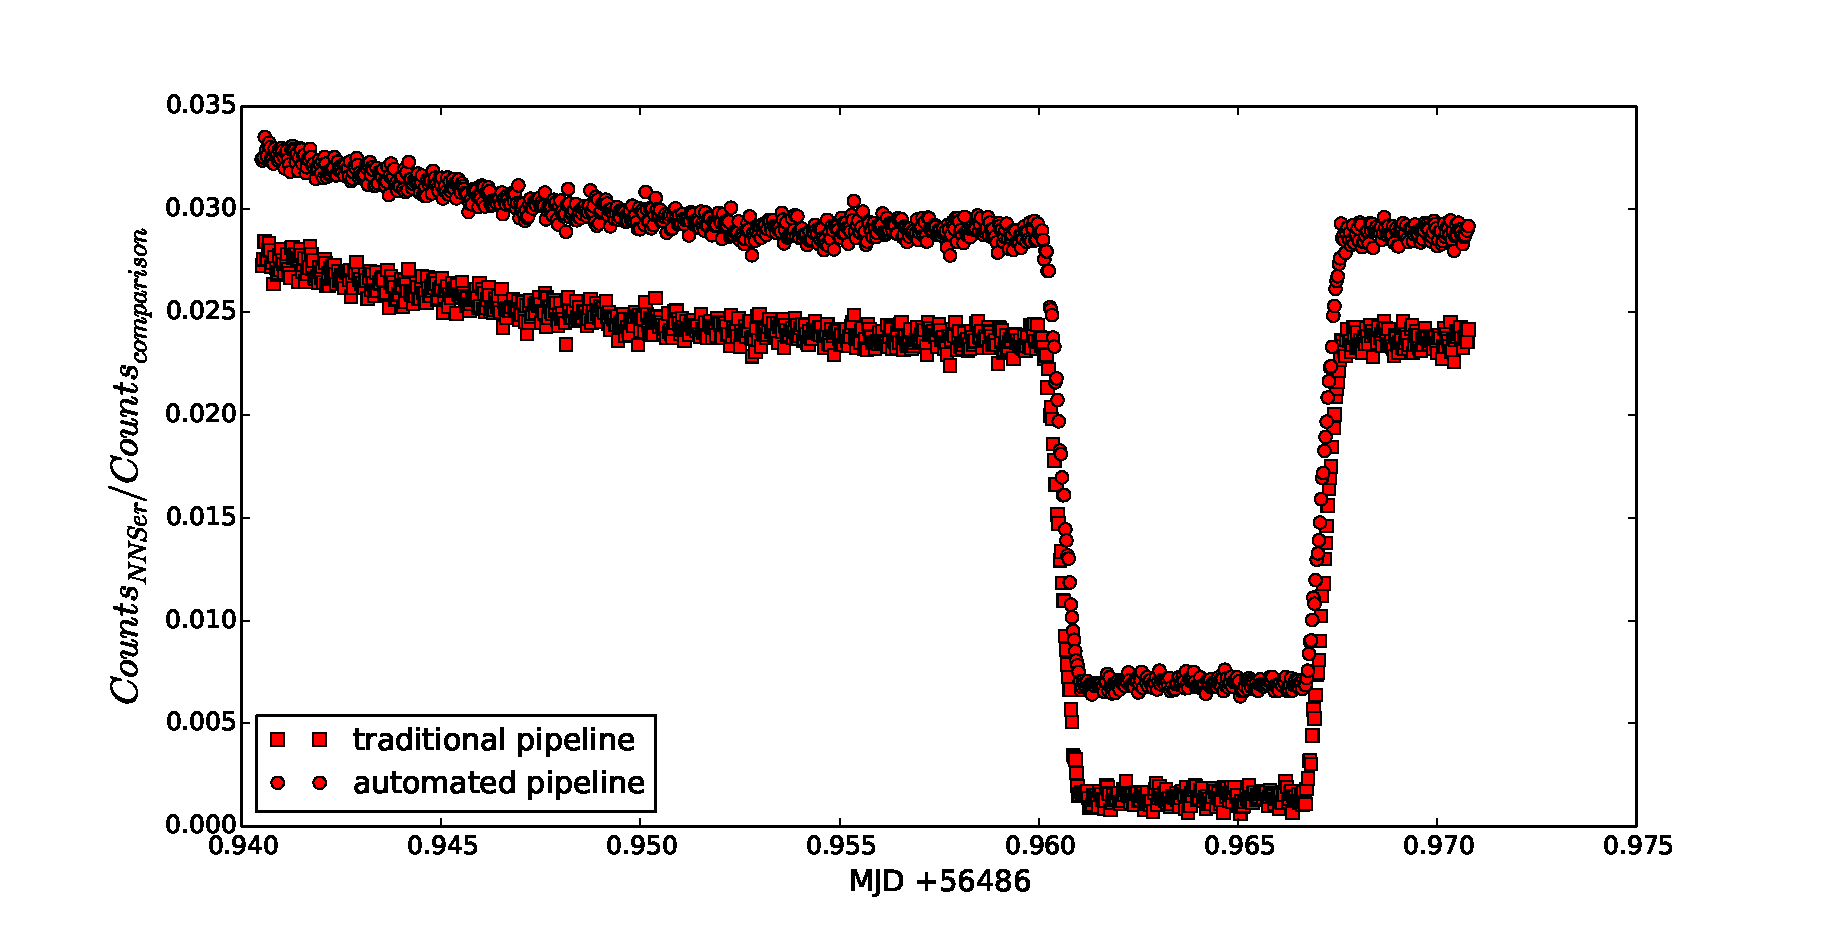
\includegraphics[width=140mm]{images/nn_ser_compare_r.eps}
\caption{Comparison of the light-curves for NN Ser in the Sloan i filter. Square data points were generated by the traditional pipeline and circles by the automated pipeline. The vertical offset applied to the circles is 0.0054. }
\label{fig:comparepipelines_r}
\end{figure}

\begin{figure}
\centering
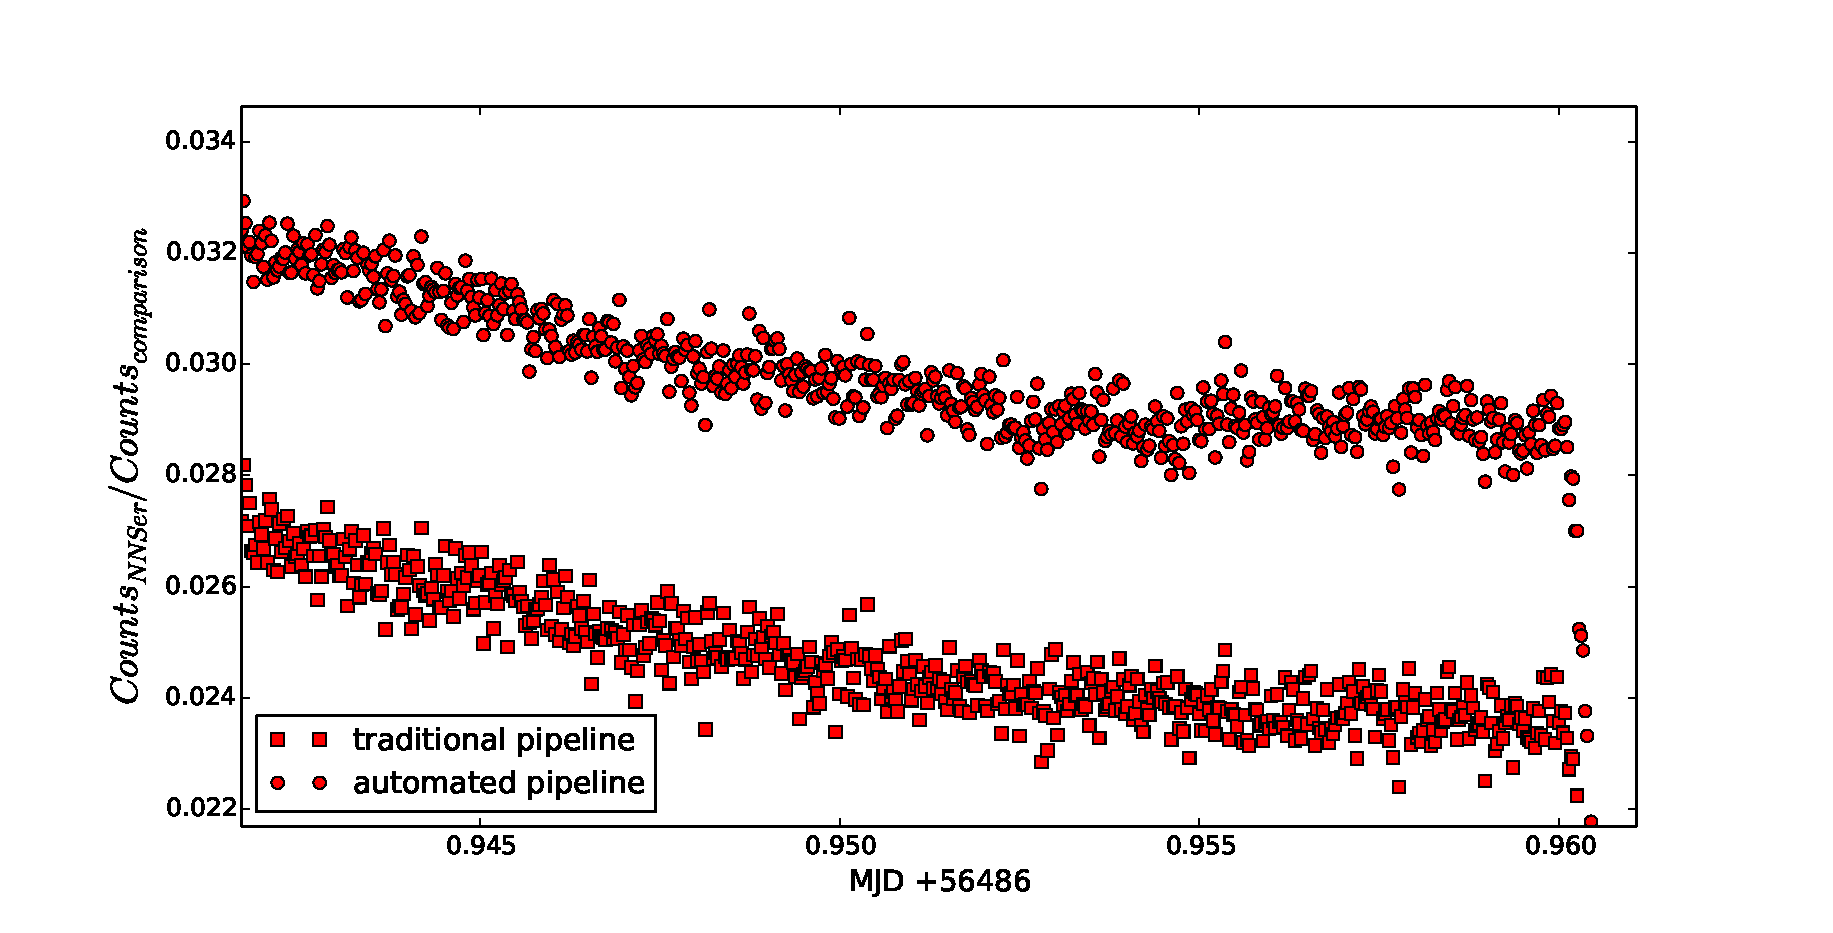
\includegraphics[width=140mm]{images/nn_ser_compare_zoom_r.eps}
\caption{A closer look at the comparison of the light-curves for NN Ser in the Sloan i filter, from the start of the run to the beginning of the eclipse ingress. Square data points were generated by the traditional pipeline and circles by the automated pipeline. The vertical offset applied to the circles is 0.0054. }
\label{fig:comparepipelines_zoom_r}
\end{figure}

\begin{figure}
\centering
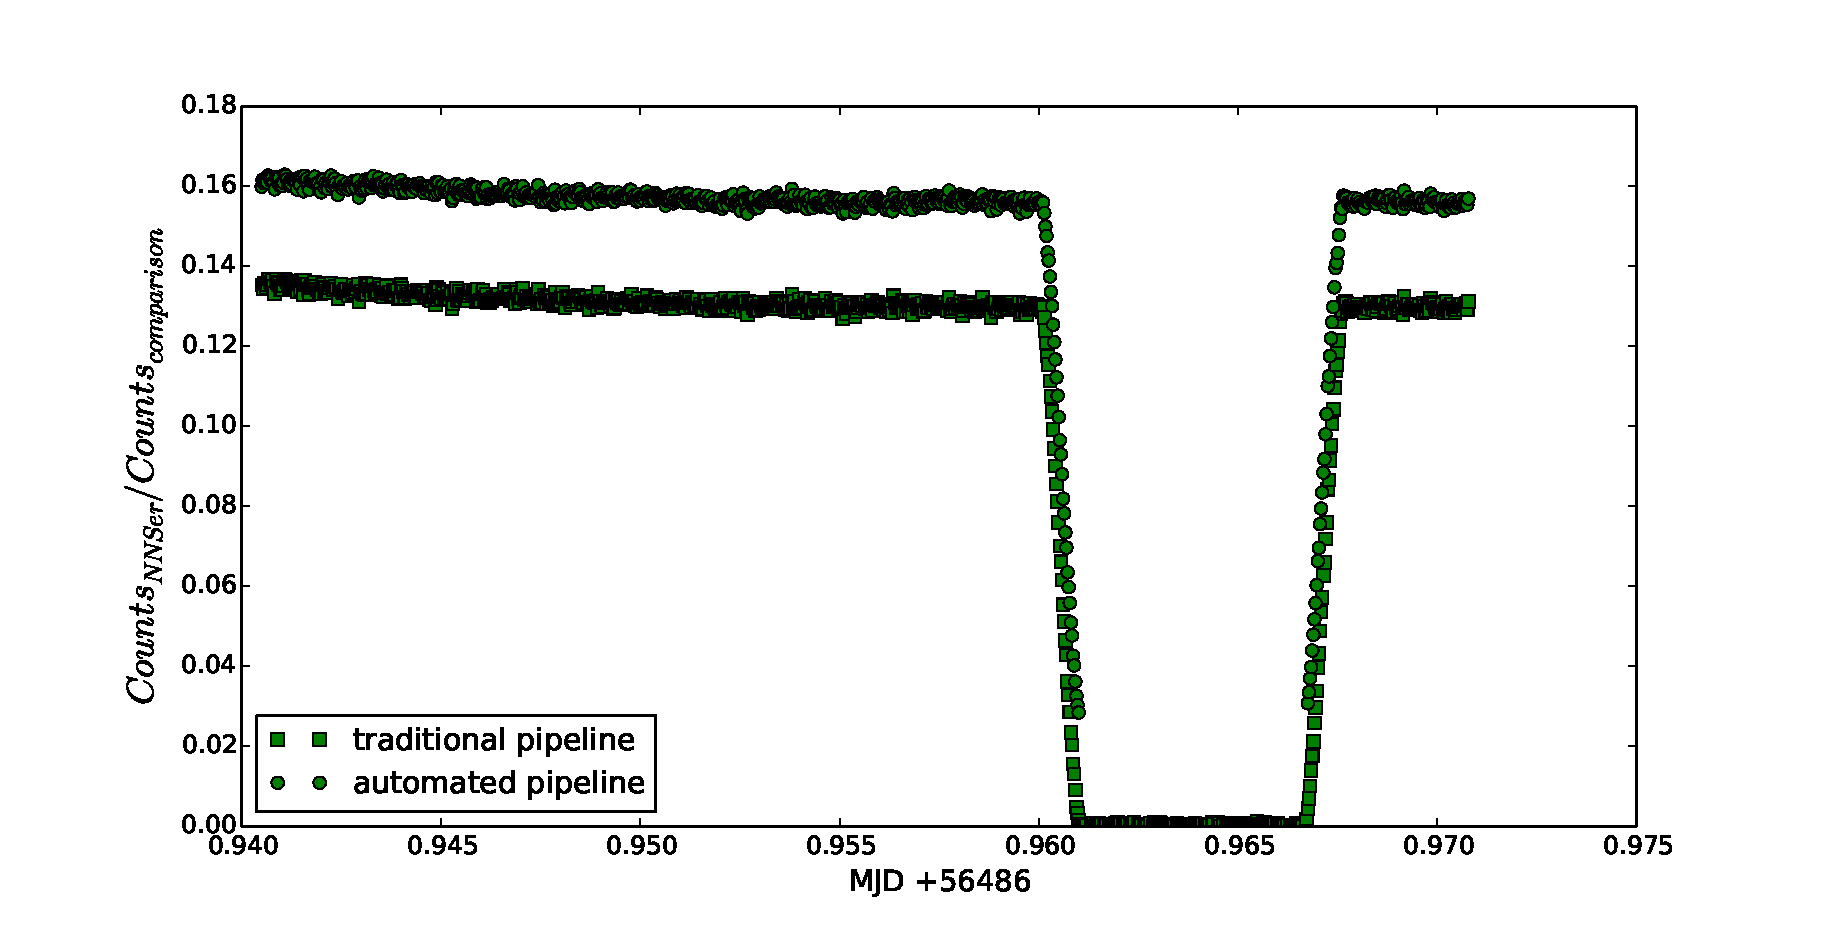
\includegraphics[width=140mm]{images/nn_ser_compare_g.eps}
\caption{Comparison of the light-curves for NN Ser in the Sloan g filter. Square data points were generated by the traditional pipeline and circles by the automated pipeline. The vertical offset applied to the circles is 0.027. Note that the automated pipeline has no data for the duration of eclipse totality. We discuss the reason for this in the text.}
\label{fig:comparepipelines_g}
\end{figure}

\begin{figure}
\centering
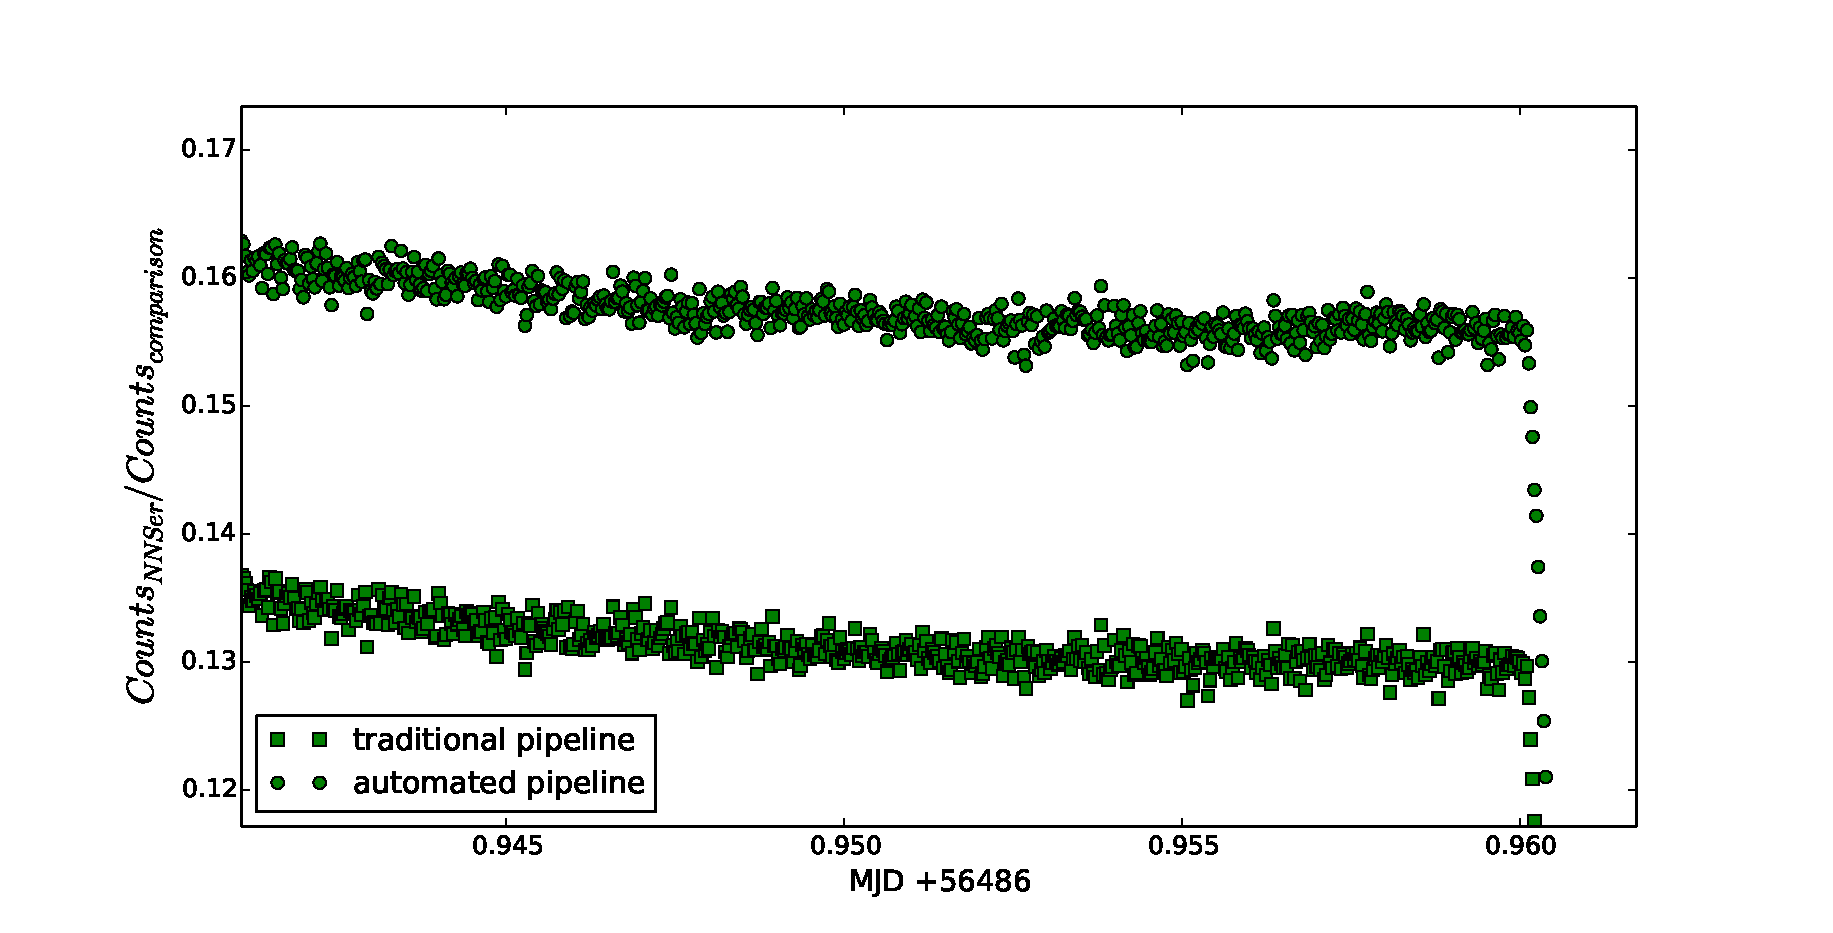
\includegraphics[width=140mm]{images/nn_ser_compare_zoom_g.eps}
\caption{A closer look at the comparison of the light-curves for NN Ser in the Sloan g filter, from the start of the run to the beginning of the eclipse ingress. Square data points were generated by the traditional pipeline and circles by the automated pipeline. The vertical offset applied to the circles is 0.027. }
\label{fig:comparepipelines_zoom_g}
\end{figure}

\begin{figure}
\centering
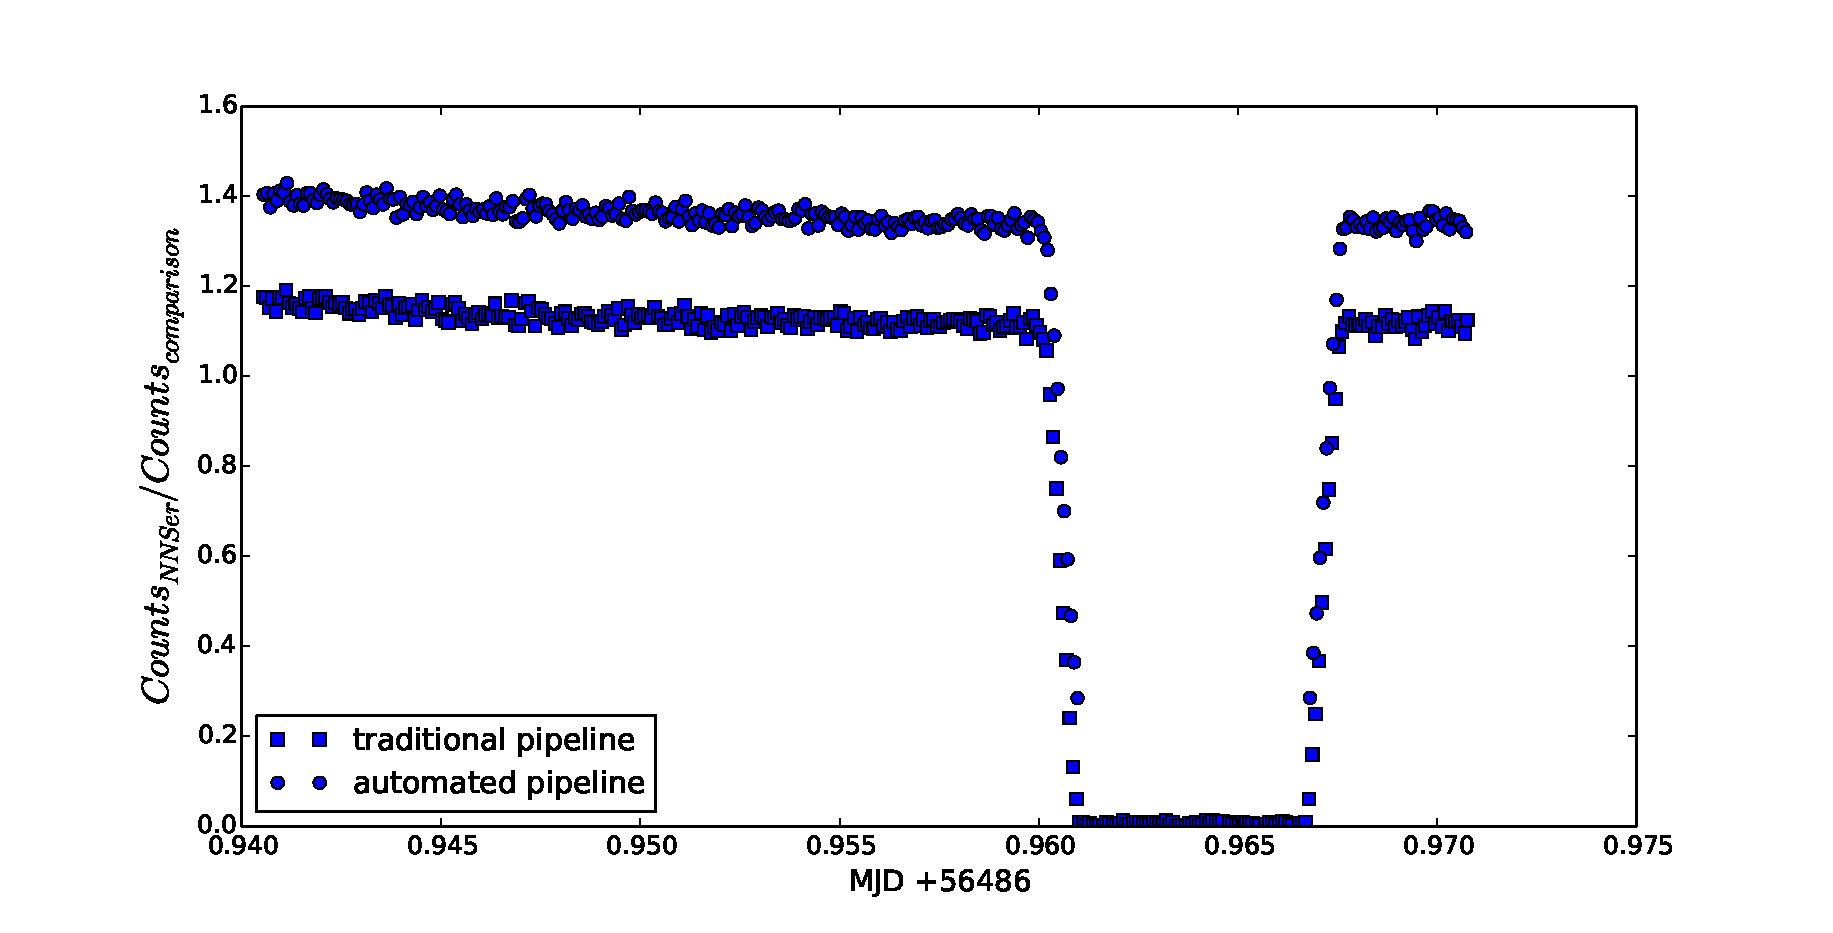
\includegraphics[width=140mm]{images/nn_ser_compare_b.eps}
\caption{Comparison of the light-curves for NN Ser in the Sloan u filter. Square data points were generated by the traditional pipeline and circles by the automated pipeline. The vertical offset applied to the circles is 0.23. Note that the automated pipeline has no data for the duration of eclipse totality. We discuss the reason for this in the text.}
\label{fig:comparepipelines_b}
\end{figure}

\begin{figure}
\centering
\includegraphics[width=140mm]{images/nn_ser_compare_zoom_b.eps}
\caption{A closer look at the comparison of the light-curves for NN Ser in the Sloan u filter, from the start of the run to the beginning of the eclipse ingress. Square data points were generated by the traditional pipeline and circles by the automated pipeline. The vertical offset applied to the circles is 0.23. }
\label{fig:comparepipelines_zoom_b}
\end{figure}

Since the automated pipeline relies on the third party software, SExtractor, to determine the apertures on each frame, objects that do not meet the required signal to noise ratio on any particular frame will not be detected and therefore have no aperture defined for that frame. No aperture means that we will have no photometry. This means that objects that fade or are generally quite faint, might disappear on some frames and then re-appear on subsequent frames. The tracking algorithm allows a re-appearing object to be identified with an object that had previously disappeared on earlier frames provided that the pixel location is roughly similar. An illustration of this can be seen in figures \ref{fig:comparepipelines_g} and \ref{fig:comparepipelines_b} where the automated pipeline loses the target object in the `g' and `u' bands after the ingress of the primary eclipse, but picks it up again at the start of egress. In contrast, the traditional reduction pipeline can have apertures that are linked to other objects in the field and can therefore continue to measure flux in the aperture for the target even if the target is barely detectable above the sky background.

% \begin{figure}
% \centering
% 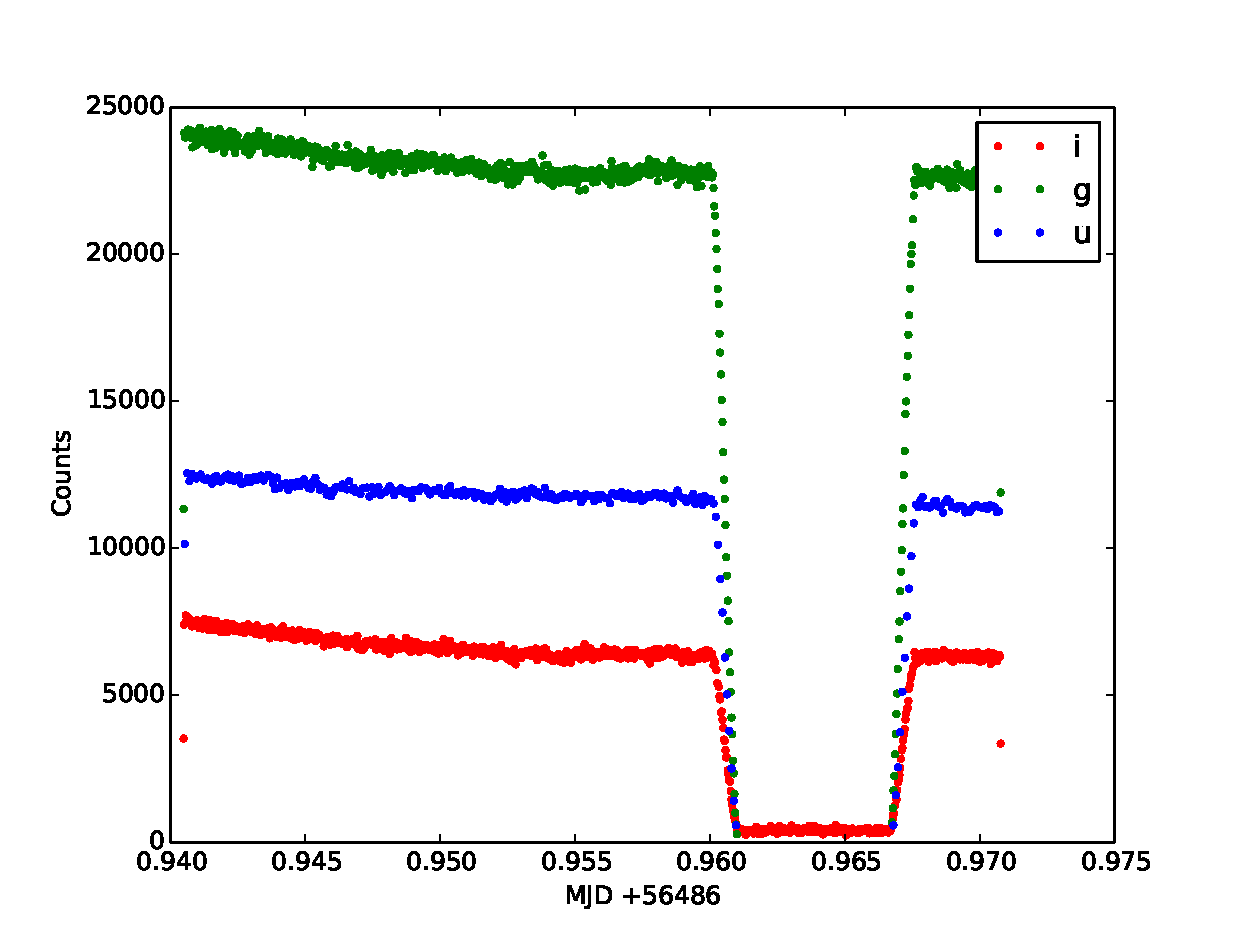
\includegraphics[width=140mm]{images/nnser_lightcurve_automated.eps}
% % % % \caption{Light curve of the target object, NN Ser produced using the \emph{automated pipeline}. The intensity of the target is plotted as its flux relative to the comparison star in the field. The red, green and blue data points are the measurements taken in the Sloan i, g, and u filters, respectively. Note that the automated pipeline (previous figure) completely loses the target in the $u$ and $g$ filters during the primary eclipse. In contrast, the traditional pipeline maintains readings of the target throughout the eclipse. This is due to the fact that the automated pipeline creates new apertures for each frame and the target is too faint during the eclipse to trigger the aperture creation for this object.}
% \label{fig:nnserlightcurveautomated}
% \end{figure}

% \begin{figure}
% \centering
% 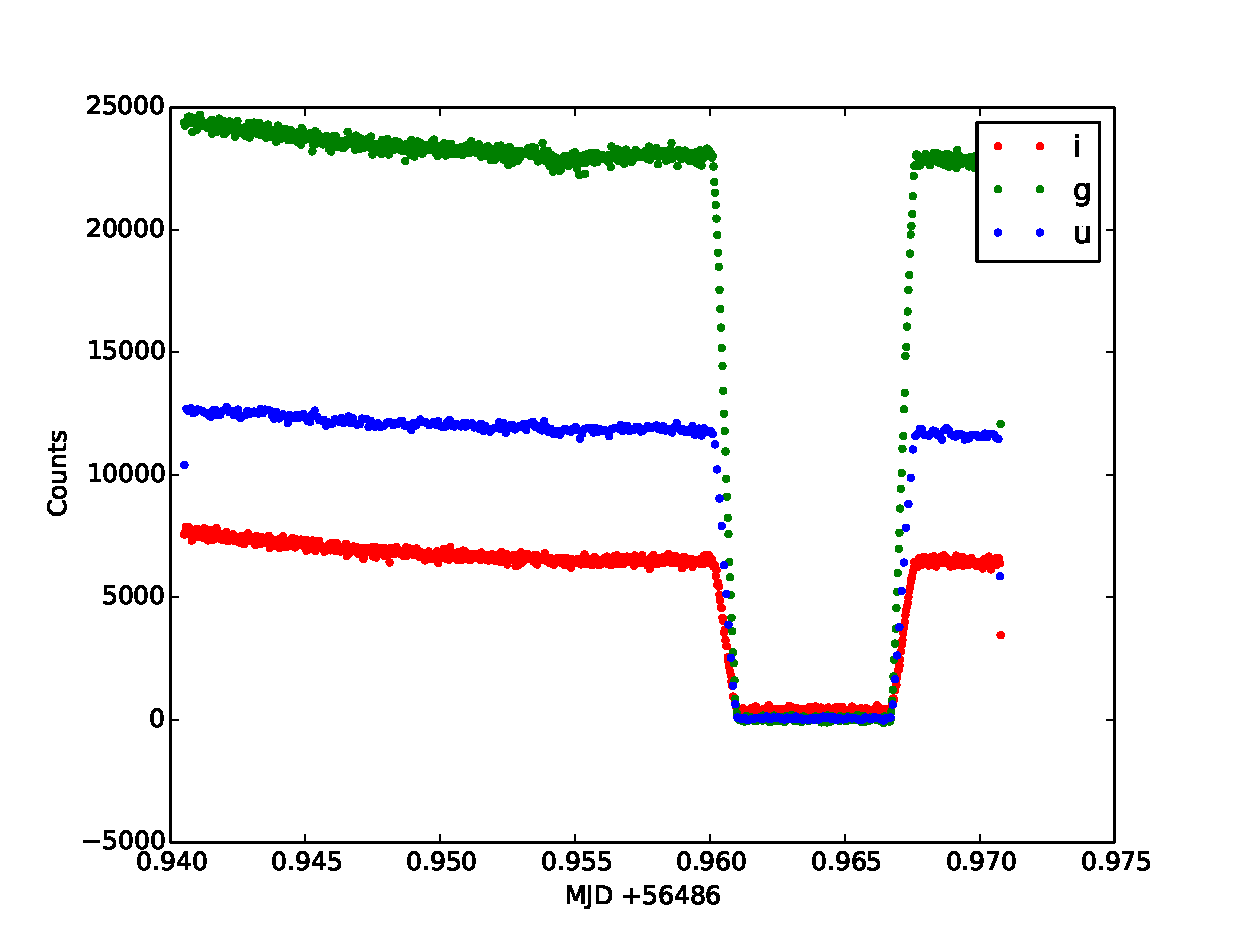
\includegraphics[width=140mm]{images/nnser_lightcurve_tom.eps}
% \caption{Light curve of the target object, NN Ser, produced using the \emph{standard pipeline}. The intensity of the target is plotted as its flux relative to the comparison star in the field. The red, green and blue data points are the measurements taken in the Sloan i, g, and u filters, respectively. }
% \label{fig:nnserlightcurvetom}
% \end{figure}

As an alternative to comparing the light-curves side-by-side we can check the systematic differences between the pipelines by comparing their measured flux values as a ratio of each other. We used both pipelines to produce light-curves for the comparison star labeled `0' in figure \ref{fig:nnserfield}. Rather than plotting each light curve separately, we have plotted the counts measured by the automated pipeline divided by the counts measured by the traditional pipeline. This is shown in figure \ref{fig:comparephotometry}. The statistics of this data set is shown in table \ref{tab:differential}. The traditional pipeline gives a slightly higher reading for the overall flux than the new automated pipeline, resulting in a mean that is less than unity. The likely cause of this is the different size of aperture used by each pipeline. This will be investigated as the pipeline is enhanced to give calibrated photometry in future versions. 

\begin{figure}
\centering
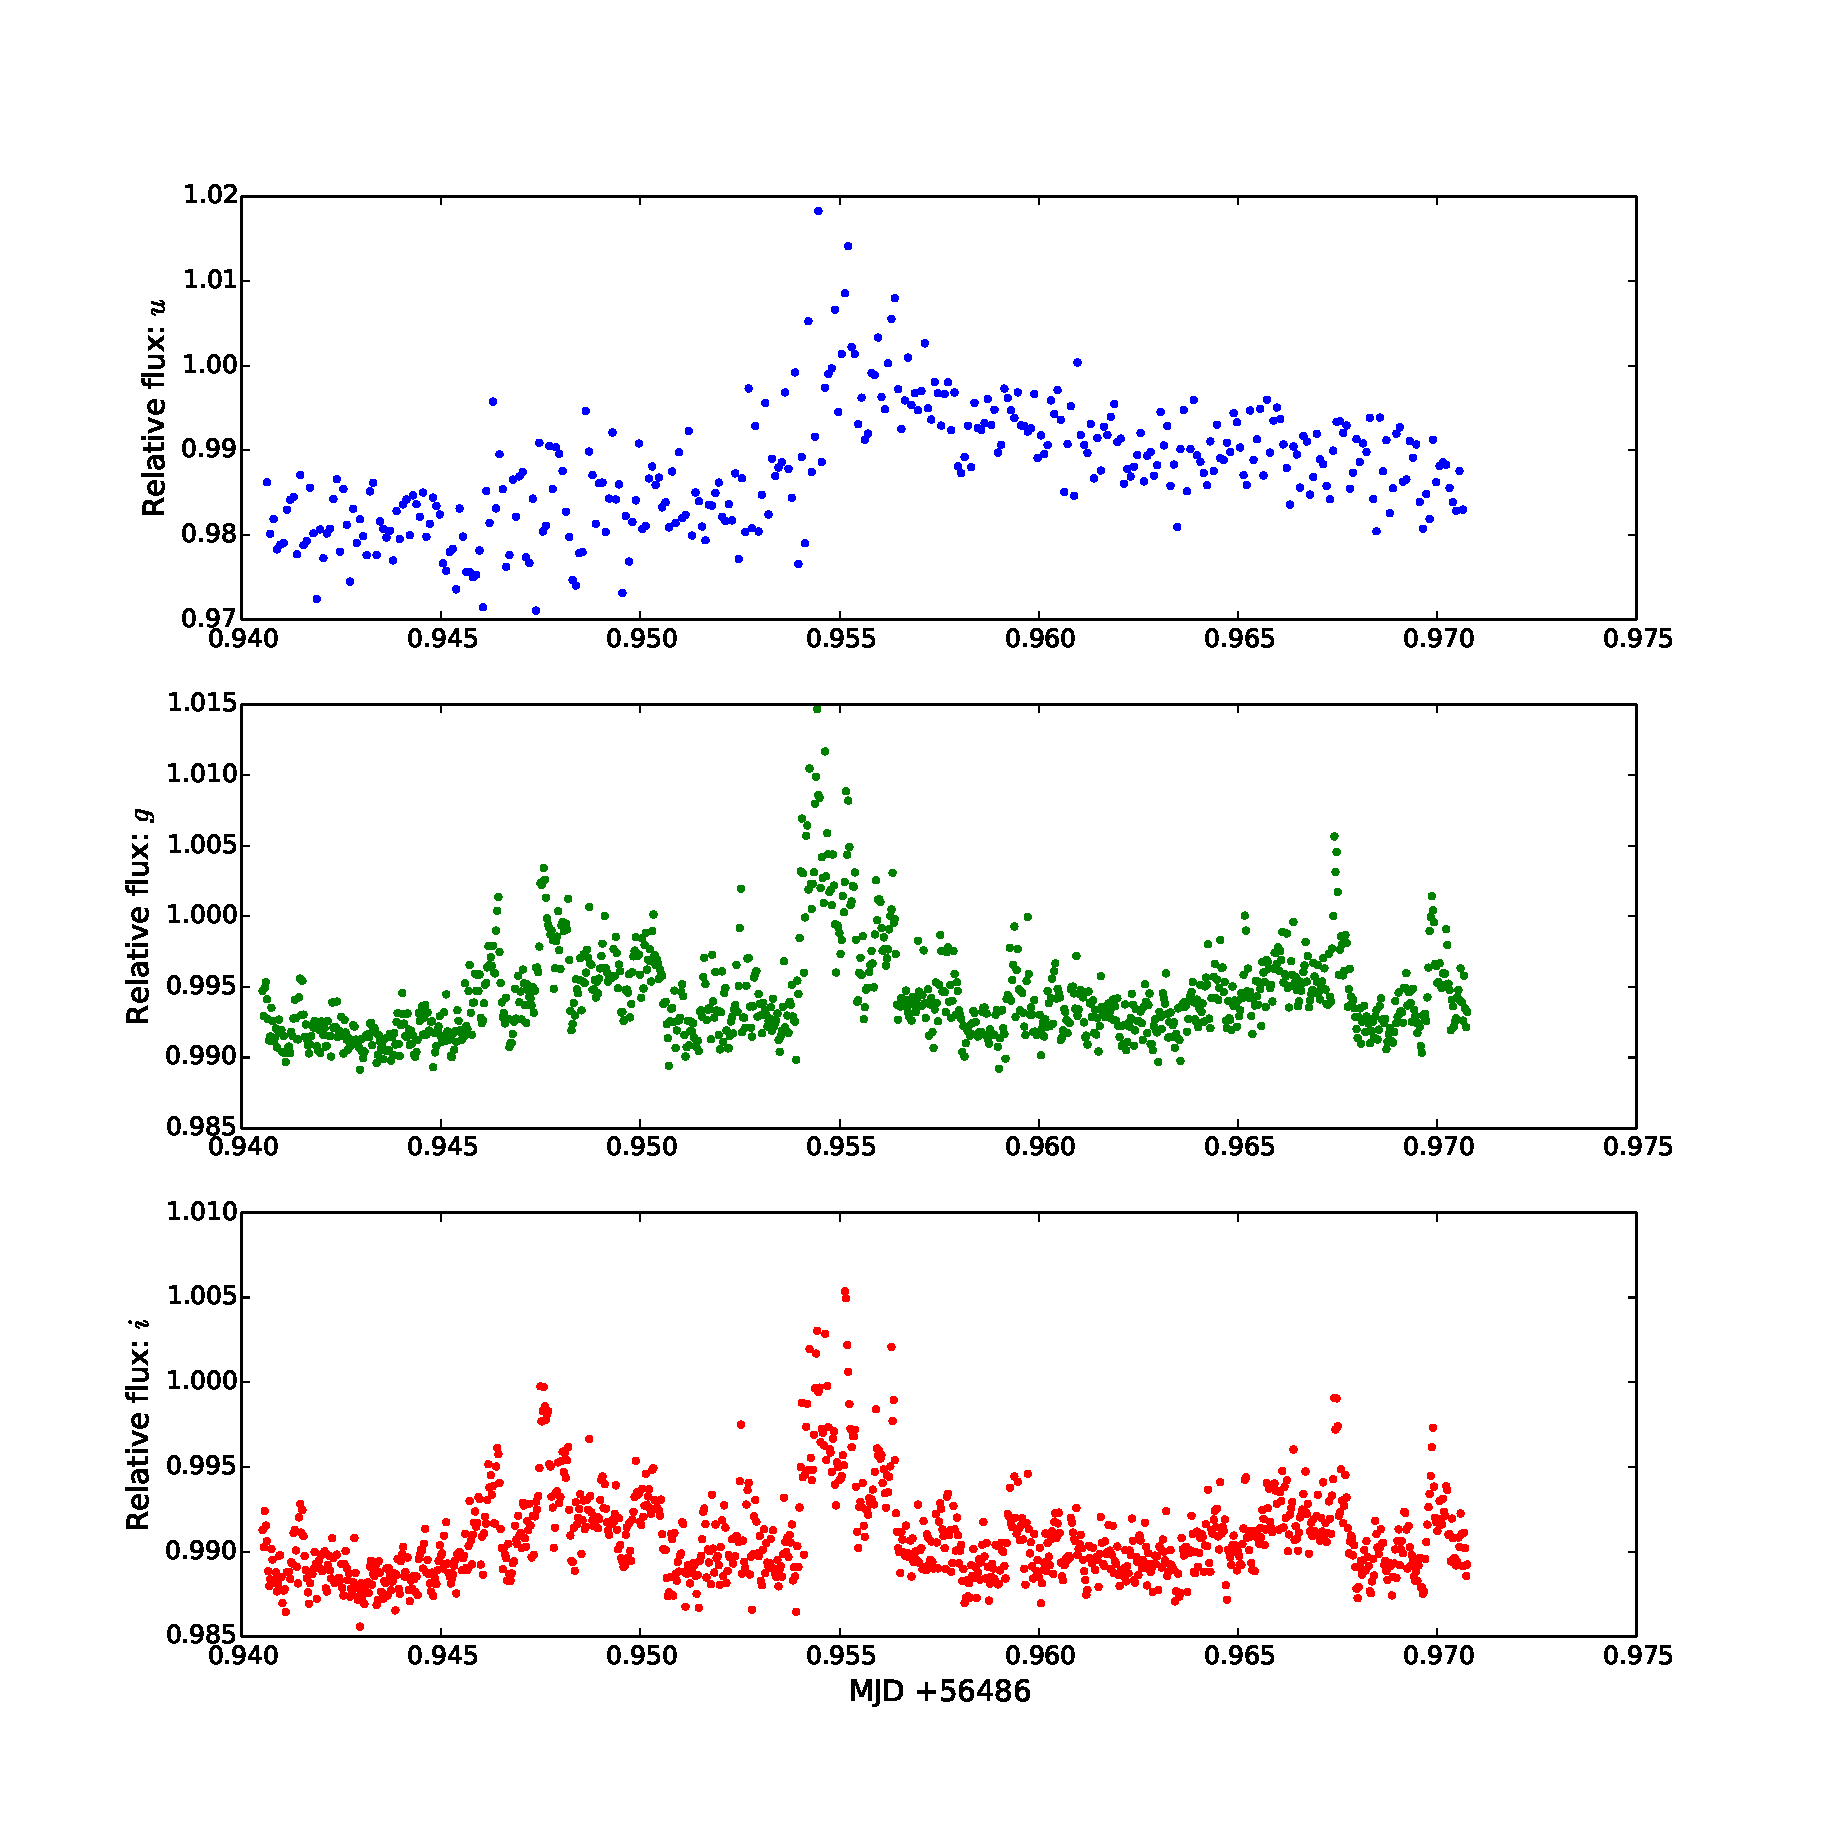
\includegraphics[width=140mm]{images/compare_photometry.eps}
\caption{A comparison of the flux measurements for a single object (object `0' in figure \ref{fig:nnserfield}). The plot is produced by dividing the flux counts as measured by the \emph{automated} pipeline by the flux counts as measured by the \emph{traditional} pipeline.}
\label{fig:comparephotometry}
\end{figure}

\begin{table}
  \centering
  \begin{tabular}{|l|r|r|}
    \hline
    Filter & Relative flux  \\
           &  $mean[std. dev]$ \\
    \hline
    'i'    & 0.991[0.003] \\
    'g'    & 0.994[0.003] \\
    'u'    & 0.988[0.007] \\
    \hline
   \end{tabular}
  \caption{Table showing the statistics of the relative photometry produced by dividing the flux counts from the automated pipeline by the flux counts from the traditional pipeline for object `0' in figure \ref{fig:nnserfield}.}
  \label{tab:differential}
  
\end{table}


\section{Object matching}
As discussed in chapter \ref{chap:datareduction}, the automated pipeline can struggle to cross-identify the same object across the different channels, r, g, b. This is usually only a problem in crowded fields where the average pixel position of the object does not clearly distinguish it from nearby objects. In other words, an object might have been identified as the same object in the blue channel (due to its proximity on the image) but is actually a near neighbour to this object in the red and green channels, so the pipeline has mistakenly assigned all three measurements as belonging to the same object.

By plotting colour-colour and colour-magnitude diagrams for a few of the crowded fields in the ULTRACAM archive we can get an indication of the severity of this mis-matching problem. Although the automated pipeline does not perform a calibration of the magnitudes of the objects, by using standard stars and extinction corrections, it is still possible to create colour-colour diagrams provided that we are not concerned with the correct offsets for our $(u-g)$ and $(g-r)$ axes. We can also produce a colour-magnitude diagram if we have a field that contains objects that are all at the same distance from us. In these automatically produced plots, there are some 'outliers' showing colours that are too extreme to be genuine astronomical bodies. 

\begin{figure}
\centering
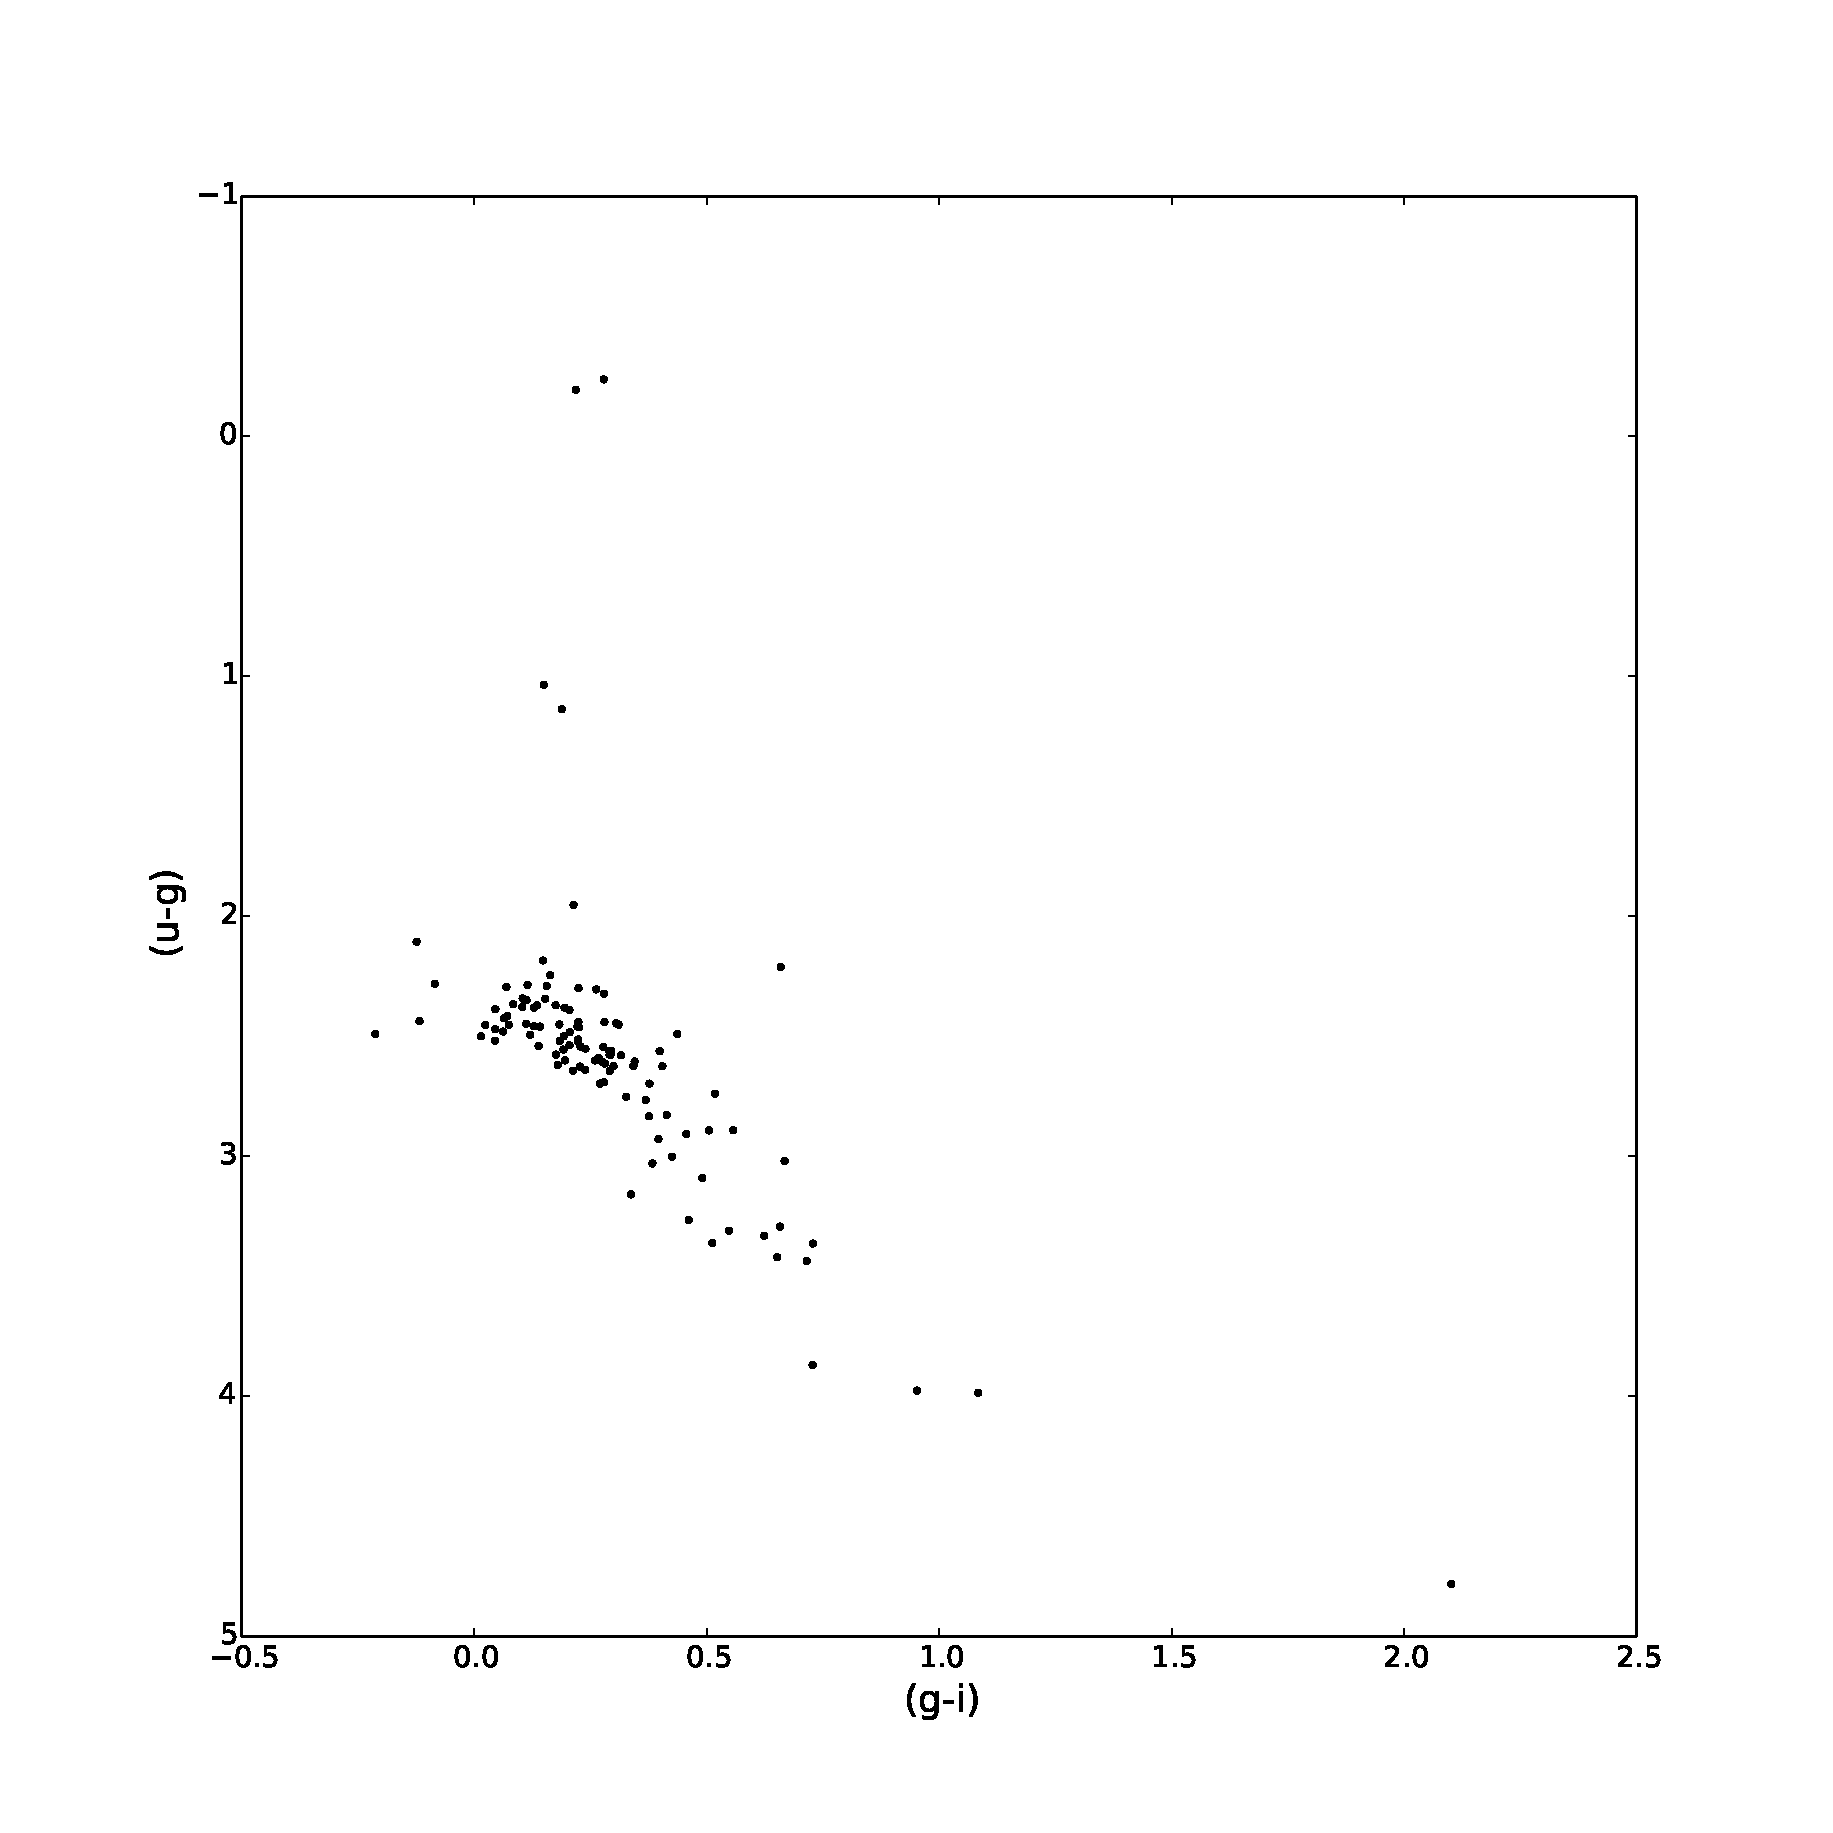
\includegraphics[width=120mm]{images/2013-07-21-run010-2colour.eps}
\caption{The colour-colour plot of run: \emph{2013-07-21/run010}. The plot contains 110 objects located near the Kepler exoplanet host KIC5115978, which is slightly out of the galactic plane. The offsets on the x and y axes are both arbitrary as the photometry has not been calibrated with photometric standards. The outliers with extreme red and blue colours are due to mistaken classification by the automated pipeline. }
\label{fig:run010-2colour}
\end{figure}

\begin{figure}
\centering
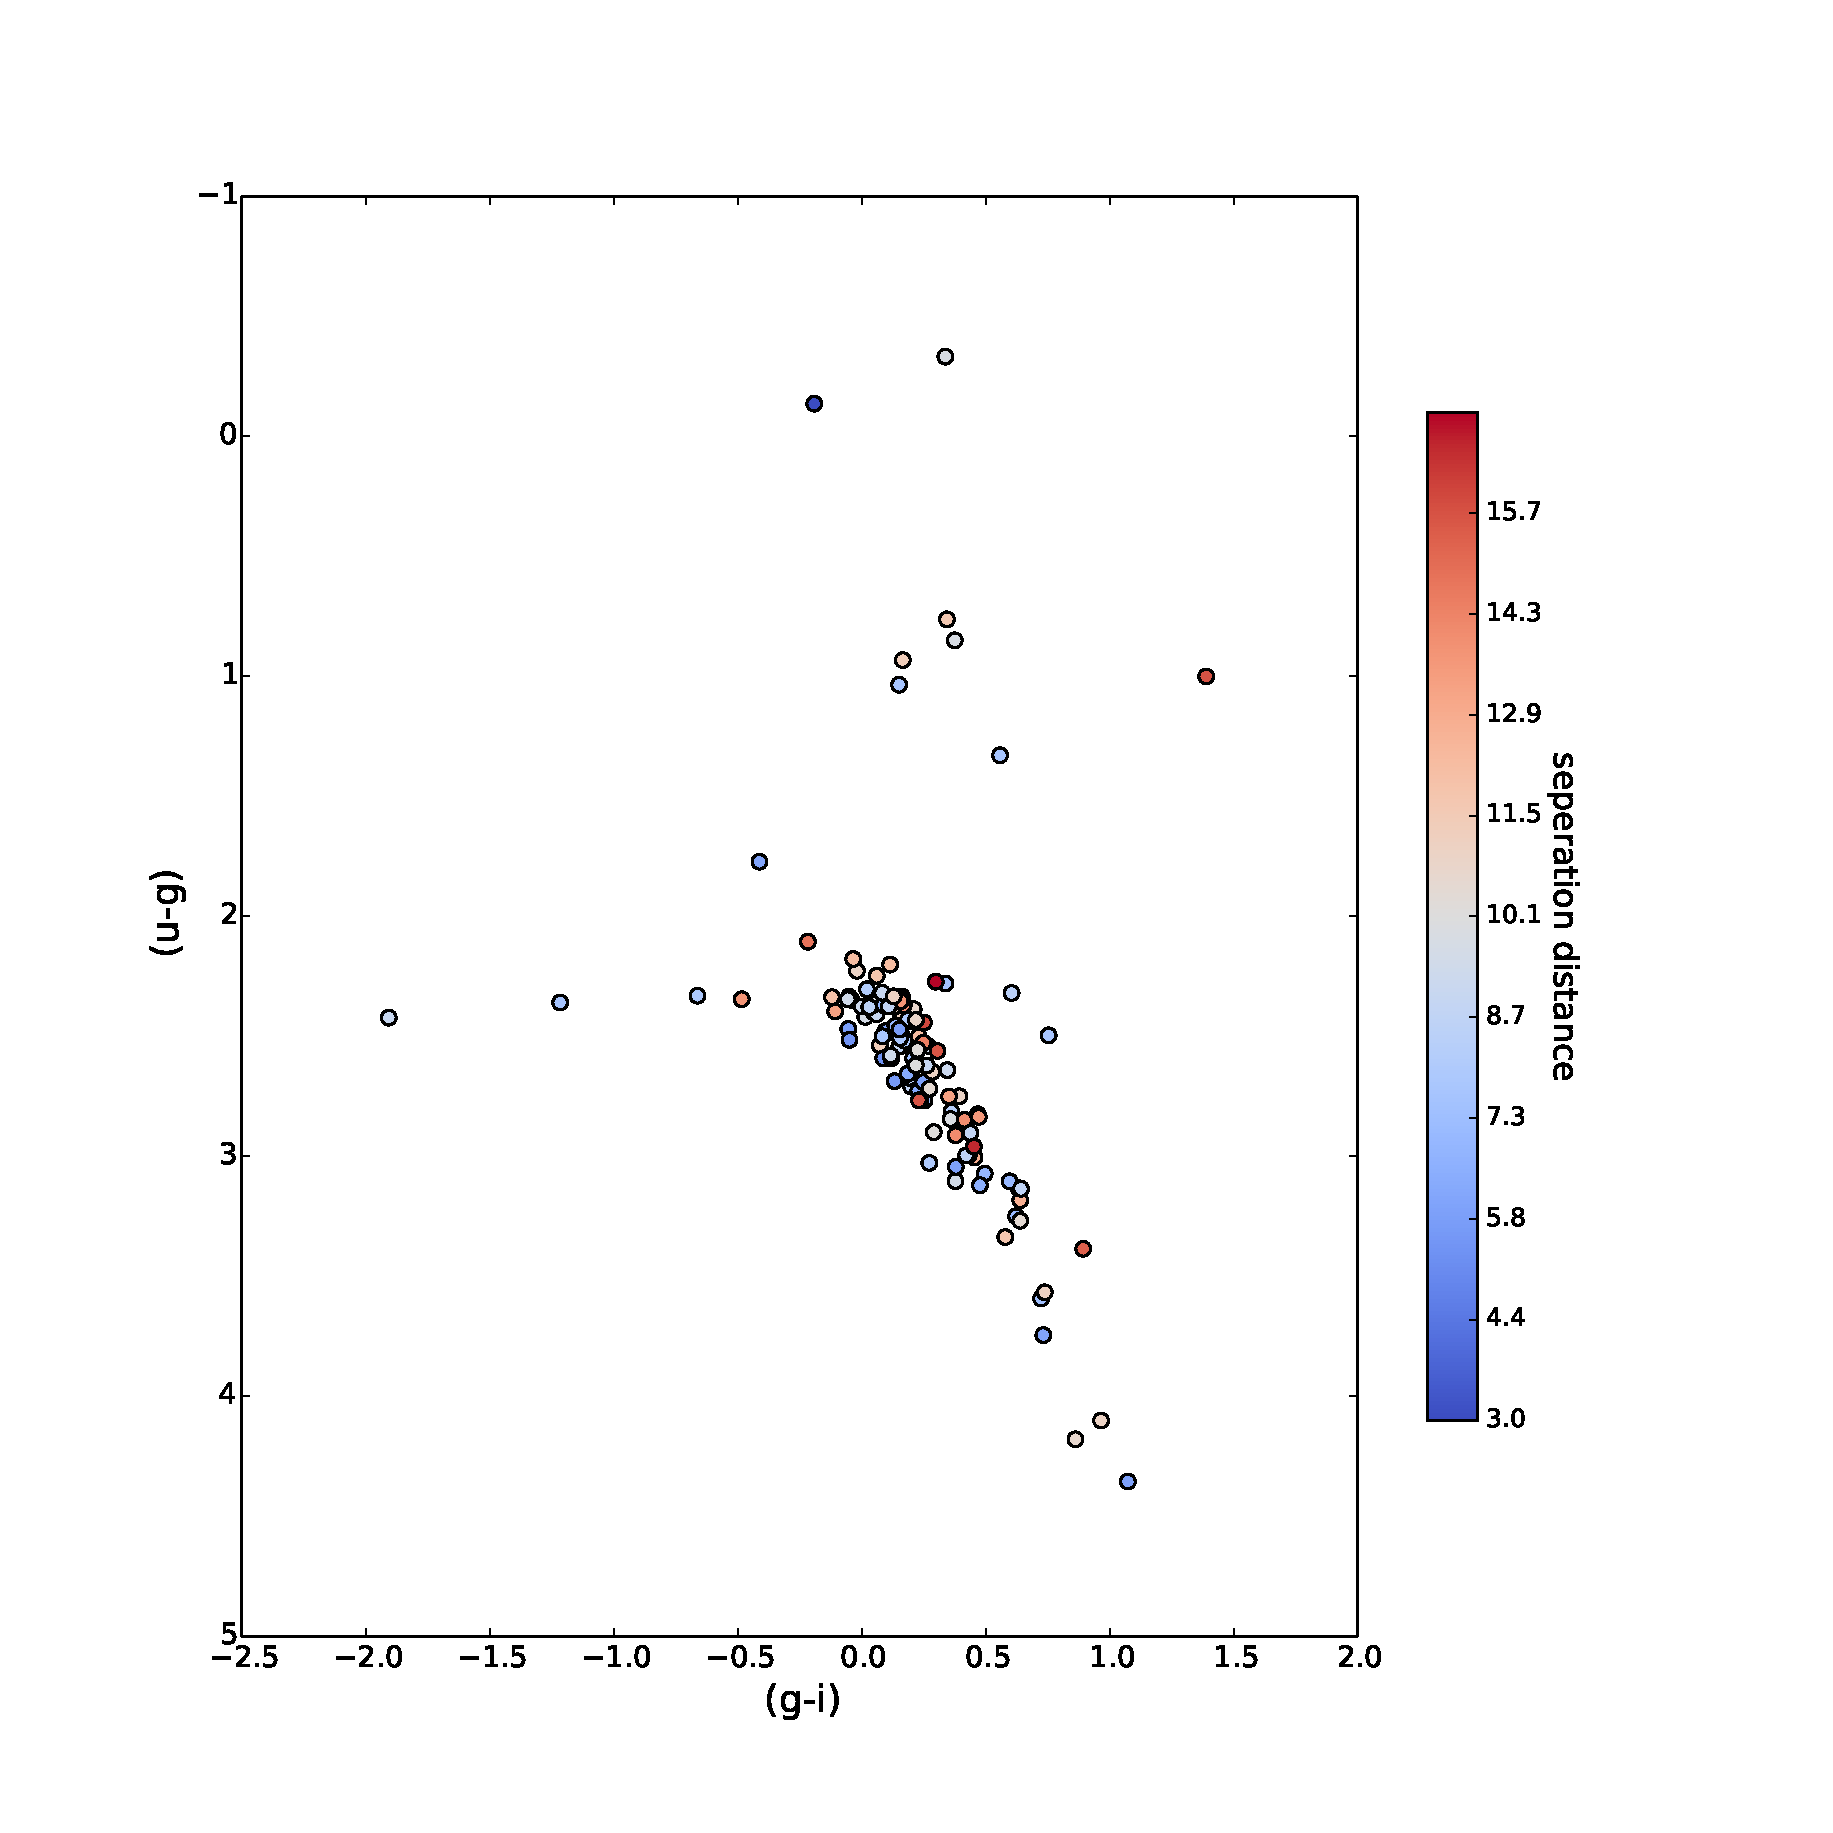
\includegraphics[width=120mm]{images/2013-07-21-run011-2colour.eps}
\caption{The colour-colour plot of run: \emph{2013-07-21/run011}. The offsets on the x and y axes are both arbitrary as the photometry has not been calibrated with photometric standards. The outliers with extreme red and blue colours are due to mistaken classification by the automated pipeline. }
\label{fig:run011-2colour}
\end{figure}


\begin{figure}
\centering
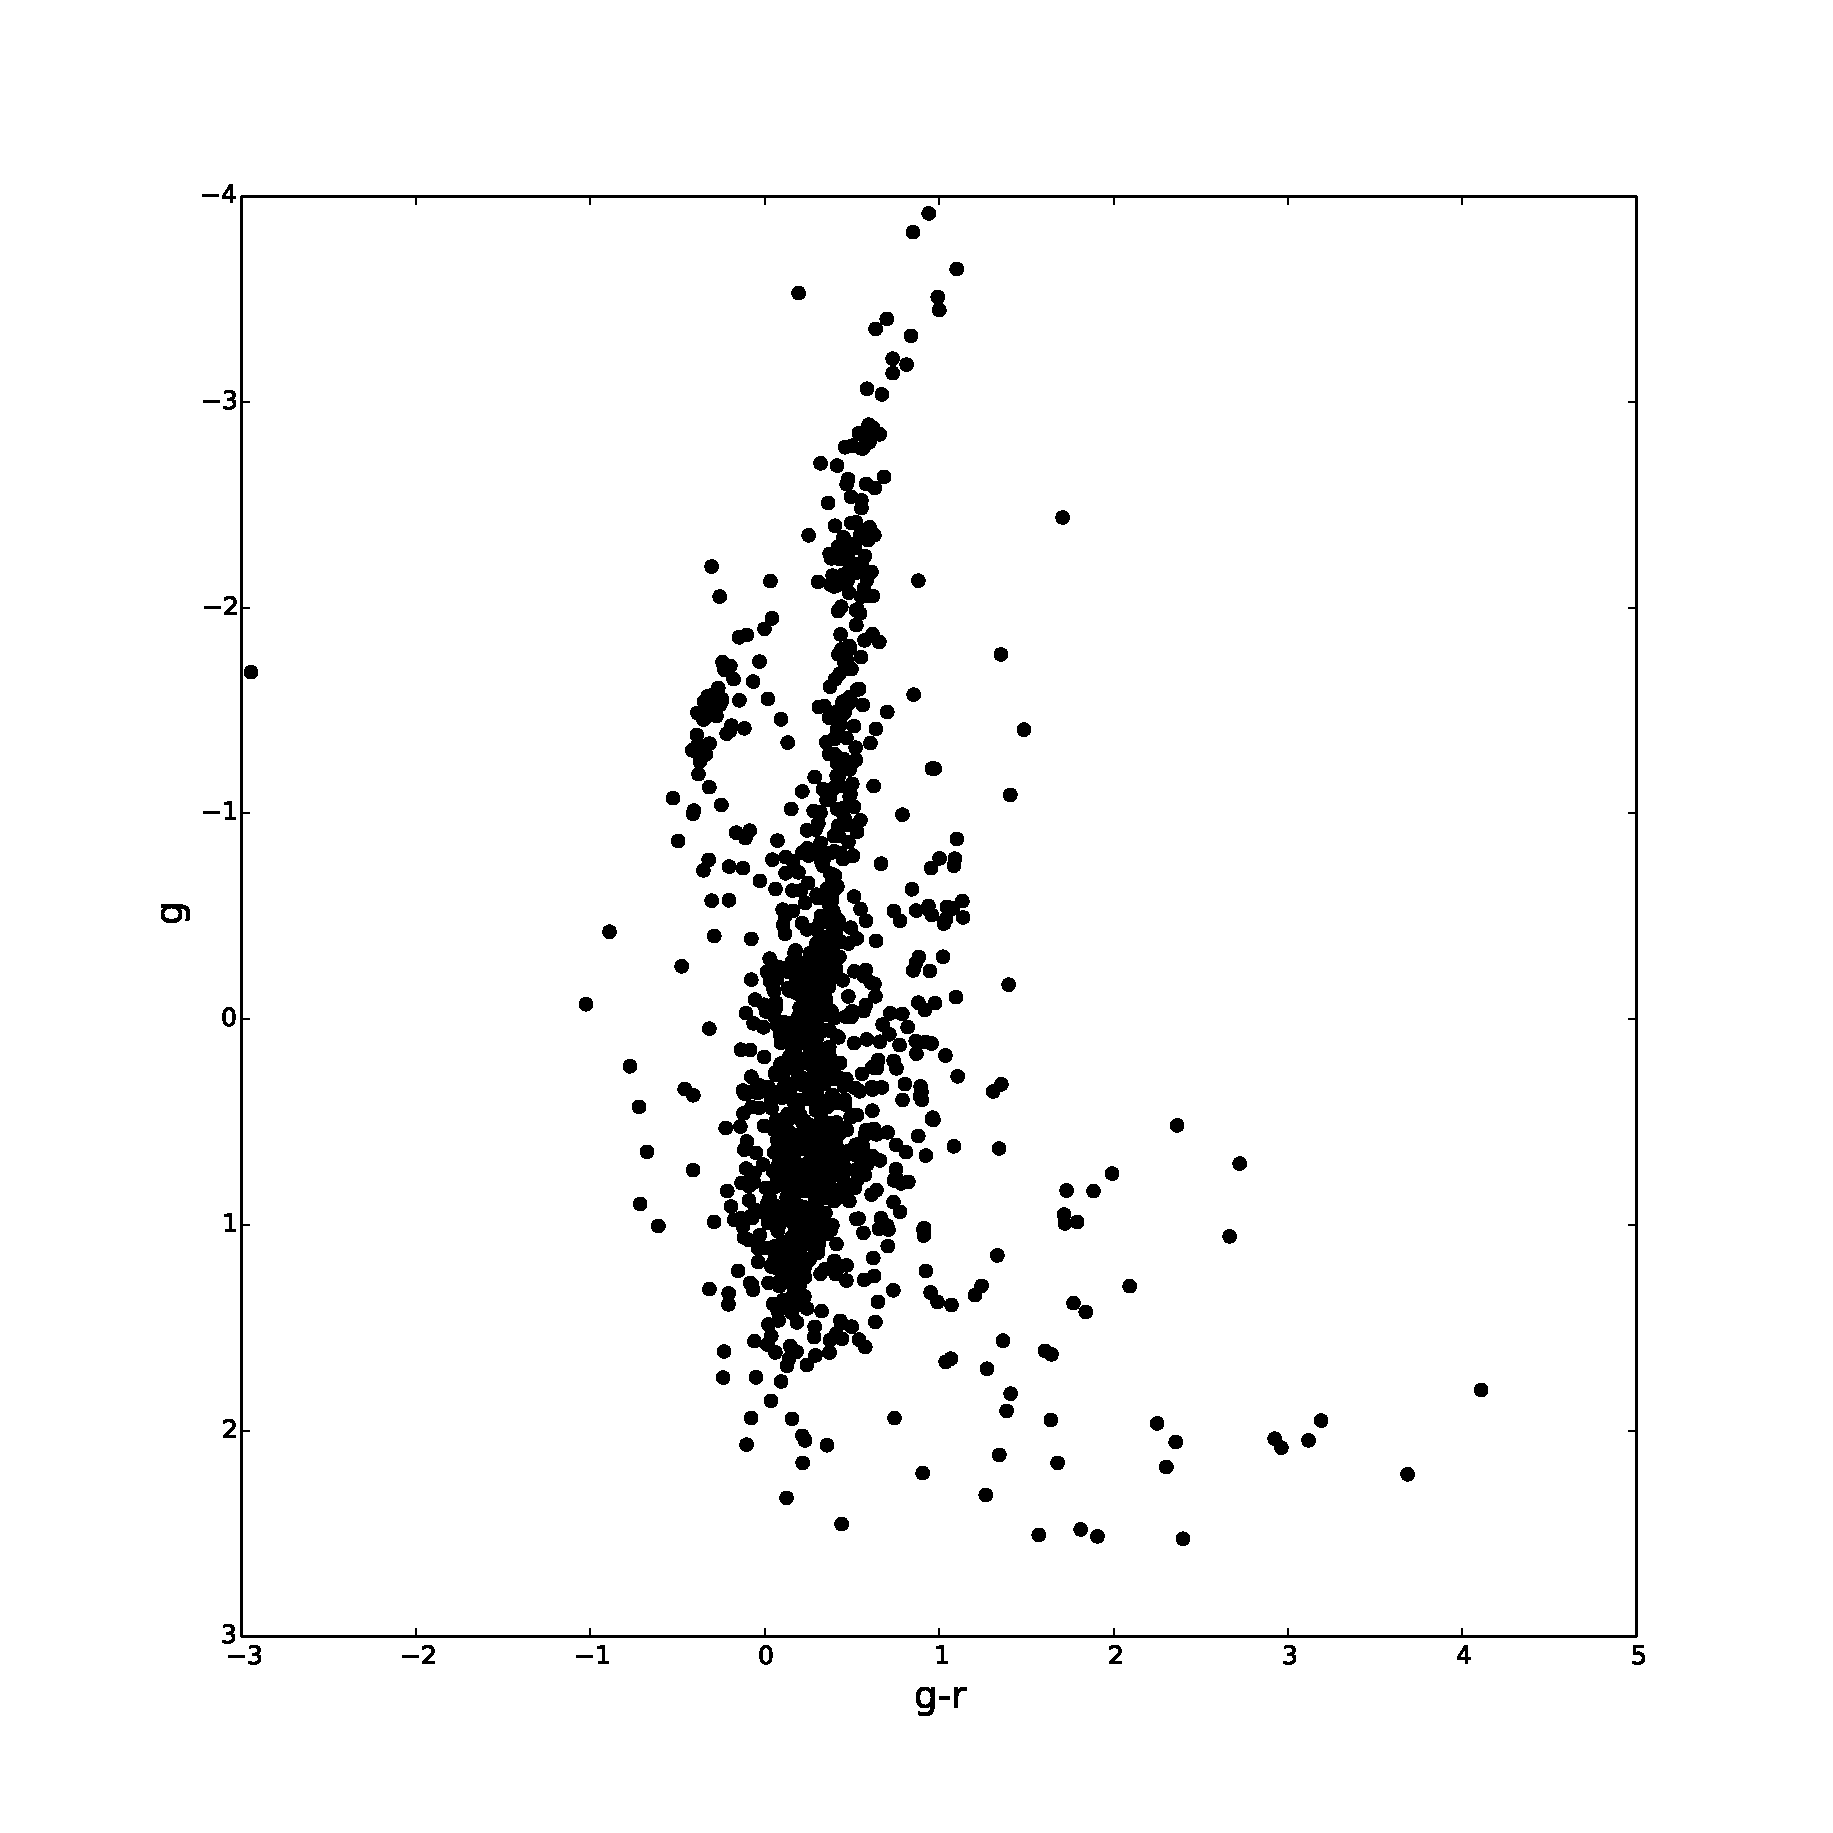
\includegraphics[width=120mm]{images//2011-04-22-run019-omegacen-colourmagnitude.eps}
\caption{A colour-magnitude plot of run: \emph{2011-04-22/run019}. The field contains 1088 objects found in a field taken of the outer perimeter of the globular cluster \emph{Omega Centaurus}. The offsets on the x and y axes are both arbitrary as the photometry has not been calibrated to photometric standards. The outliers with extreme red and blue colours are due to mistaken classification by the automated pipeline.}
\label{fig:OmegaCen-colourmagnitude}
\end{figure}

\section{Processing the entire ULTRACAM archive}
In order to make the processing of the ULTRACAM archive as free from manual intervention as possible, a few additional scripts were written to coordinate the steps of the pipeline as described in the previous two chapters. These wrapper scripts were designed to trigger the pipeline for a full day's worth of data with a single command. The University of Warwick has a high performance computing facility called `Cluster of Workstations' (CoWS) that uses idle computing time on all of the desktop machines in the department. A script was written that sends the automated pipeline processing jobs to this shared facility. Using this approach, it was possible to process nearly all of the ULTRACAM archive in about 2 weeks. At present \emph{347} nights, out of a total of \emph{406}, have been processed and are available for viewing on a web server hosted at the University of Warwick. 

The runs that have not been processed are a few very high cadence runs with exposure times of less than 0.1 seconds and numbers of frames exceeding 50,000. The automated pipeline can take more than 8 hours of processing time for these runs. Using the Cluster of Workstations is possible to continue to process these runs. However, it was felt that a different  and more optimised version of the pipeline should be built to treat these runs differently, rather than using brute-force to process them. These runs usually have very few objects in the fields, typically only the target object and the comparison and this situation is handled very well by the traditional pipeline. The processing of high cadence runs with very few objects was not a goal for this project. 

Of these 347 nights, approximately 20\% of the science runs have been investigated for objects with variability. The method of investigation is to perform by a visual check of the light-curve. The web interface is designed such that it is easy for the viewer to examine the light-curves of all of the objects systematically. The user-interface allows the users to see each light curve in turn by pressing the 'right' and 'left'  arrow keys on the keyboard. More information on how to use this interface can be found in the User Manual, appendix ~\ref{chap:usermanual}. 
